\documentclass[12pt]{article}

%packages
%\usepackage{latexsym}
\usepackage{graphicx}
\usepackage{color}
\usepackage{amsmath}
\usepackage{dsfont}
\usepackage{placeins}
\usepackage{amssymb}
\usepackage{wasysym}
\usepackage{abstract}
\usepackage{hyperref}
\usepackage{etoolbox}
\usepackage{datetime}
\usepackage{xcolor}
\usepackage{alphalph}
\settimeformat{ampmtime}

%\usepackage{pstricks,pst-node,pst-tree}

%\usepackage{algpseudocode}
%\usepackage{amsthm}
%\usepackage{hyperref}
%\usepackage{mathrsfs}
%\usepackage{amsfonts}
%\usepackage{bbding}
%\usepackage{listings}
%\usepackage{appendix}
\usepackage[margin=1in]{geometry}
%\geometry{papersize={8.5in,11in},total={6.5in,9in}}
%\usepackage{cancel}
%\usepackage{algorithmic, algorithm}

\makeatletter
\def\maxwidth{ %
  \ifdim\Gin@nat@width>\linewidth
    \linewidth
  \else
    \Gin@nat@width
  \fi
}
\makeatother

\definecolor{fgcolor}{rgb}{0.345, 0.345, 0.345}
\newcommand{\hlnum}[1]{\textcolor[rgb]{0.686,0.059,0.569}{#1}}%
\newcommand{\hlstr}[1]{\textcolor[rgb]{0.192,0.494,0.8}{#1}}%
\newcommand{\hlcom}[1]{\textcolor[rgb]{0.678,0.584,0.686}{\textit{#1}}}%
\newcommand{\hlopt}[1]{\textcolor[rgb]{0,0,0}{#1}}%
\newcommand{\hlstd}[1]{\textcolor[rgb]{0.345,0.345,0.345}{#1}}%
\newcommand{\hlkwa}[1]{\textcolor[rgb]{0.161,0.373,0.58}{\textbf{#1}}}%
\newcommand{\hlkwb}[1]{\textcolor[rgb]{0.69,0.353,0.396}{#1}}%
\newcommand{\hlkwc}[1]{\textcolor[rgb]{0.333,0.667,0.333}{#1}}%
\newcommand{\hlkwd}[1]{\textcolor[rgb]{0.737,0.353,0.396}{\textbf{#1}}}%

\usepackage{framed}
\makeatletter
\newenvironment{kframe}{%
 \def\at@end@of@kframe{}%
 \ifinner\ifhmode%
  \def\at@end@of@kframe{\end{minipage}}%
  \begin{minipage}{\columnwidth}%
 \fi\fi%
 \def\FrameCommand##1{\hskip\@totalleftmargin \hskip-\fboxsep
 \colorbox{shadecolor}{##1}\hskip-\fboxsep
     % There is no \\@totalrightmargin, so:
     \hskip-\linewidth \hskip-\@totalleftmargin \hskip\columnwidth}%
 \MakeFramed {\advance\hsize-\width
   \@totalleftmargin\z@ \linewidth\hsize
   \@setminipage}}%
 {\par\unskip\endMakeFramed%
 \at@end@of@kframe}
\makeatother

\definecolor{shadecolor}{rgb}{.77, .77, .77}
\definecolor{messagecolor}{rgb}{0, 0, 0}
\definecolor{warningcolor}{rgb}{1, 0, 1}
\definecolor{errorcolor}{rgb}{1, 0, 0}
\newenvironment{knitrout}{}{} % an empty environment to be redefined in TeX

\usepackage{alltt}
\usepackage[T1]{fontenc}

\newcommand{\qu}[1]{``#1''}
\newcounter{probnum}
\setcounter{probnum}{1}

%create definition to allow local margin changes
\def\changemargin#1#2{\list{}{\rightmargin#2\leftmargin#1}\item[]}
\let\endchangemargin=\endlist 

%allow equations to span multiple pages
\allowdisplaybreaks

%define colors and color typesetting conveniences
\definecolor{gray}{rgb}{0.5,0.5,0.5}
\definecolor{black}{rgb}{0,0,0}
\definecolor{white}{rgb}{1,1,1}
\definecolor{blue}{rgb}{0.5,0.5,1}
\newcommand{\inblue}[1]{\color{blue}#1 \color{black}}
\definecolor{green}{rgb}{0.133,0.545,0.133}
\newcommand{\ingreen}[1]{\color{green}#1 \color{black}}
\definecolor{yellow}{rgb}{1,1,0}
\newcommand{\inyellow}[1]{\color{yellow}#1 \color{black}}
\definecolor{orange}{rgb}{0.9,0.649,0}
\newcommand{\inorange}[1]{\color{orange}#1 \color{black}}
\definecolor{red}{rgb}{1,0.133,0.133}
\newcommand{\inred}[1]{\color{red}#1 \color{black}}
\definecolor{purple}{rgb}{0.58,0,0.827}
\newcommand{\inpurple}[1]{\color{purple}#1 \color{black}}
\definecolor{backgcode}{rgb}{0.97,0.97,0.8}
\definecolor{Brown}{cmyk}{0,0.81,1,0.60}
\definecolor{OliveGreen}{cmyk}{0.64,0,0.95,0.40}
\definecolor{CadetBlue}{cmyk}{0.62,0.57,0.23,0}

%define new math operators
\DeclareMathOperator*{\argmax}{arg\,max~}
\DeclareMathOperator*{\argmin}{arg\,min~}
\DeclareMathOperator*{\argsup}{arg\,sup~}
\DeclareMathOperator*{\arginf}{arg\,inf~}
\DeclareMathOperator*{\convolution}{\text{\Huge{$\ast$}}}
\newcommand{\infconv}[2]{\convolution^\infty_{#1 = 1} #2}
%true functions

%%%% GENERAL SHORTCUTS

%shortcuts for pure typesetting conveniences
\newcommand{\bv}[1]{\boldsymbol{#1}}

%shortcuts for compound constants
\newcommand{\BetaDistrConst}{\dfrac{\Gamma(\alpha + \beta)}{\Gamma(\alpha)\Gamma(\beta)}}
\newcommand{\NormDistrConst}{\dfrac{1}{\sqrt{2\pi\sigma^2}}}

%shortcuts for conventional symbols
\newcommand{\tsq}{\tau^2}
\newcommand{\tsqh}{\hat{\tau}^2}
\newcommand{\sigsq}{\sigma^2}
\newcommand{\sigsqsq}{\parens{\sigma^2}^2}
\newcommand{\sigsqovern}{\dfrac{\sigsq}{n}}
\newcommand{\tausq}{\tau^2}
\newcommand{\tausqalpha}{\tau^2_\alpha}
\newcommand{\tausqbeta}{\tau^2_\beta}
\newcommand{\tausqsigma}{\tau^2_\sigma}
\newcommand{\betasq}{\beta^2}
\newcommand{\sigsqvec}{\bv{\sigma}^2}
\newcommand{\sigsqhat}{\hat{\sigma}^2}
\newcommand{\sigsqhatmlebayes}{\sigsqhat_{\text{Bayes, MLE}}}
\newcommand{\sigsqhatmle}[1]{\sigsqhat_{#1, \text{MLE}}}
\newcommand{\bSigma}{\bv{\Sigma}}
\newcommand{\bSigmainv}{\bSigma^{-1}}
\newcommand{\thetavec}{\bv{\theta}}
\newcommand{\thetahat}{\hat{\theta}}
\newcommand{\thetahatmle}{\hat{\theta}_{\mathrm{MLE}}}
\newcommand{\thetavechatmle}{\hat{\thetavec}_{\mathrm{MLE}}}
\newcommand{\muhat}{\hat{\mu}}
\newcommand{\musq}{\mu^2}
\newcommand{\muvec}{\bv{\mu}}
\newcommand{\muhatmle}{\muhat_{\text{MLE}}}
\newcommand{\lambdahat}{\hat{\lambda}}
\newcommand{\lambdahatmle}{\lambdahat_{\text{MLE}}}
\newcommand{\etavec}{\bv{\eta}}
\newcommand{\alphavec}{\bv{\alpha}}
\newcommand{\minimaxdec}{\delta^*_{\mathrm{mm}}}
\newcommand{\ybar}{\bar{y}}
\newcommand{\xbar}{\bar{x}}
\newcommand{\Xbar}{\bar{X}}
\newcommand{\phat}{\hat{p}}
\newcommand{\Phat}{\hat{P}}
\newcommand{\Zbar}{\bar{Z}}
\newcommand{\iid}{~{\buildrel iid \over \sim}~}
\newcommand{\inddist}{~{\buildrel ind \over \sim}~}
\newcommand{\approxdist}{~{\buildrel approx \over \sim}~}
\newcommand{\equalsindist}{~{\buildrel d \over =}~}
\newcommand{\loglik}[1]{\ell\parens{#1}}
\newcommand{\thetahatkminone}{\thetahat^{(k-1)}}
\newcommand{\thetahatkplusone}{\thetahat^{(k+1)}}
\newcommand{\thetahatk}{\thetahat^{(k)}}
\newcommand{\half}{\frac{1}{2}}
\newcommand{\third}{\frac{1}{3}}
\newcommand{\twothirds}{\frac{2}{3}}
\newcommand{\fourth}{\frac{1}{4}}
\newcommand{\fifth}{\frac{1}{5}}
\newcommand{\sixth}{\frac{1}{6}}

%shortcuts for vector and matrix notation
\newcommand{\A}{\bv{A}}
\newcommand{\At}{\A^T}
\newcommand{\Ainv}{\inverse{\A}}
\newcommand{\B}{\bv{B}}
\newcommand{\K}{\bv{K}}
\newcommand{\Kt}{\K^T}
\newcommand{\Kinv}{\inverse{K}}
\newcommand{\Kinvt}{(\Kinv)^T}
\newcommand{\M}{\bv{M}}
\newcommand{\Bt}{\B^T}
\newcommand{\Q}{\bv{Q}}
\newcommand{\Qt}{\Q^T}
\newcommand{\R}{\bv{R}}
\newcommand{\Rt}{\R^T}
\newcommand{\Z}{\bv{Z}}
\newcommand{\X}{\bv{X}}
\newcommand{\Xsub}{\X_{\text{(sub)}}}
\newcommand{\Xsubadj}{\X_{\text{(sub,adj)}}}
\newcommand{\I}{\bv{I}}
\newcommand{\Y}{\bv{Y}}
\newcommand{\T}{\bv{T}}
\newcommand{\sigsqI}{\sigsq\I}
\renewcommand{\P}{\bv{P}}
\newcommand{\Psub}{\P_{\text{(sub)}}}
\newcommand{\Pt}{\P^T}
\newcommand{\Pii}{P_{ii}}
\newcommand{\Pij}{P_{ij}}
\newcommand{\IminP}{(\I-\P)}
\newcommand{\Xt}{\bv{X}^T}
\newcommand{\XtX}{\Xt\X}
\newcommand{\XtXinv}{\parens{\Xt\X}^{-1}}
\newcommand{\XtXinvXt}{\XtXinv\Xt}
\newcommand{\XXtXinvXt}{\X\XtXinvXt}
\newcommand{\x}{\bv{x}}
\newcommand{\p}{\bv{p}}
\newcommand{\onevec}{\bv{1}}
\newcommand{\oneton}{1, \ldots, n}
\newcommand{\yoneton}{y_1, \ldots, y_n}
\newcommand{\yonetonorder}{y_{(1)}, \ldots, y_{(n)}}
\newcommand{\Yoneton}{Y_1, \ldots, Y_n}
\newcommand{\iinoneton}{i \in \braces{\oneton}}
\newcommand{\onetom}{1, \ldots, m}
\newcommand{\jinonetom}{j \in \braces{\onetom}}
\newcommand{\xoneton}{x_1, \ldots, x_n}
\newcommand{\Xoneton}{X_1, \ldots, X_n}
\newcommand{\xt}{\x^T}
\newcommand{\y}{\bv{y}}
\newcommand{\yt}{\y^T}
\renewcommand{\c}{\bv{c}}
\newcommand{\ct}{\c^T}
\newcommand{\tstar}{\bv{t}^*}
\renewcommand{\u}{\bv{u}}
\renewcommand{\v}{\bv{v}}
\renewcommand{\a}{\bv{a}}
\newcommand{\s}{\bv{s}}
\newcommand{\yadj}{\y_{\text{(adj)}}}
\newcommand{\xjadj}{\x_{j\text{(adj)}}}
\newcommand{\xjadjM}{\x_{j \perp M}}
\newcommand{\yhat}{\hat{\y}}
\newcommand{\yhatsub}{\yhat_{\text{(sub)}}}
\newcommand{\yhatstar}{\yhat^*}
\newcommand{\yhatstarnew}{\yhatstar_{\text{new}}}
\newcommand{\z}{\bv{z}}
\newcommand{\zt}{\z^T}
\newcommand{\bb}{\bv{b}}
\newcommand{\bbt}{\bb^T}
\newcommand{\bbeta}{\bv{\beta}}
\newcommand{\beps}{\bv{\epsilon}}
\newcommand{\bepst}{\beps^T}
\newcommand{\e}{\bv{e}}
\newcommand{\Mofy}{\M(\y)}
\newcommand{\KofAlpha}{K(\alpha)}
\newcommand{\ellset}{\mathcal{L}}
\newcommand{\oneminalph}{1-\alpha}
\newcommand{\SSE}{\text{SSE}}
\newcommand{\SSEsub}{\text{SSE}_{\text{(sub)}}}
\newcommand{\MSE}{\text{MSE}}
\newcommand{\RMSE}{\text{RMSE}}
\newcommand{\SSR}{\text{SSR}}
\newcommand{\SST}{\text{SST}}
\newcommand{\JSest}{\delta_{\text{JS}}(\x)}
\newcommand{\Bayesest}{\delta_{\text{Bayes}}(\x)}
\newcommand{\EmpBayesest}{\delta_{\text{EmpBayes}}(\x)}
\newcommand{\BLUPest}{\delta_{\text{BLUP}}}
\newcommand{\MLEest}[1]{\hat{#1}_{\text{MLE}}}

%shortcuts for Linear Algebra stuff (i.e. vectors and matrices)
\newcommand{\twovec}[2]{\bracks{\begin{array}{c} #1 \\ #2 \end{array}}}
\newcommand{\threevec}[3]{\bracks{\begin{array}{c} #1 \\ #2 \\ #3 \end{array}}}
\newcommand{\fivevec}[5]{\bracks{\begin{array}{c} #1 \\ #2 \\ #3 \\ #4 \\ #5 \end{array}}}
\newcommand{\twobytwomat}[4]{\bracks{\begin{array}{cc} #1 & #2 \\ #3 & #4 \end{array}}}
\newcommand{\threebytwomat}[6]{\bracks{\begin{array}{cc} #1 & #2 \\ #3 & #4 \\ #5 & #6 \end{array}}}

%shortcuts for conventional compound symbols
\newcommand{\thetainthetas}{\theta \in \Theta}
\newcommand{\reals}{\mathbb{R}}
\newcommand{\complexes}{\mathbb{C}}
\newcommand{\rationals}{\mathbb{Q}}
\newcommand{\integers}{\mathbb{Z}}
\newcommand{\naturals}{\mathbb{N}}
\newcommand{\forallninN}{~~\forall n \in \naturals}
\newcommand{\forallxinN}[1]{~~\forall #1 \in \reals}
\newcommand{\matrixdims}[2]{\in \reals^{\,#1 \times #2}}
\newcommand{\inRn}[1]{\in \reals^{\,#1}}
\newcommand{\mathimplies}{\quad\Rightarrow\quad}
\newcommand{\mathlogicequiv}{\quad\Leftrightarrow\quad}
\newcommand{\eqncomment}[1]{\quad \text{(#1)}}
\newcommand{\limitn}{\lim_{n \rightarrow \infty}}
\newcommand{\limitN}{\lim_{N \rightarrow \infty}}
\newcommand{\limitd}{\lim_{d \rightarrow \infty}}
\newcommand{\limitt}{\lim_{t \rightarrow \infty}}
\newcommand{\limitsupn}{\limsup_{n \rightarrow \infty}~}
\newcommand{\limitinfn}{\liminf_{n \rightarrow \infty}~}
\newcommand{\limitk}{\lim_{k \rightarrow \infty}}
\newcommand{\limsupn}{\limsup_{n \rightarrow \infty}}
\newcommand{\limsupk}{\limsup_{k \rightarrow \infty}}
\newcommand{\floor}[1]{\left\lfloor #1 \right\rfloor}
\newcommand{\ceil}[1]{\left\lceil #1 \right\rceil}

%shortcuts for environments
\newcommand{\beqn}{\vspace{-0.25cm}\begin{eqnarray*}}
\newcommand{\eeqn}{\end{eqnarray*}}
\newcommand{\bneqn}{\vspace{-0.25cm}\begin{eqnarray}}
\newcommand{\eneqn}{\end{eqnarray}}

%shortcuts for mini environments
\newcommand{\parens}[1]{\left(#1\right)}
\newcommand{\squared}[1]{\parens{#1}^2}
\newcommand{\tothepow}[2]{\parens{#1}^{#2}}
\newcommand{\prob}[1]{\mathbb{P}\parens{#1}}
\newcommand{\cprob}[2]{\prob{#1~|~#2}}
\newcommand{\littleo}[1]{o\parens{#1}}
\newcommand{\bigo}[1]{O\parens{#1}}
\newcommand{\Lp}[1]{\mathbb{L}^{#1}}
\renewcommand{\arcsin}[1]{\text{arcsin}\parens{#1}}
\newcommand{\prodonen}[2]{\bracks{\prod_{#1=1}^n #2}}
\newcommand{\mysum}[4]{\sum_{#1=#2}^{#3} #4}
\newcommand{\sumonen}[2]{\sum_{#1=1}^n #2}
\newcommand{\infsum}[2]{\sum_{#1=1}^\infty #2}
\newcommand{\infprod}[2]{\prod_{#1=1}^\infty #2}
\newcommand{\infunion}[2]{\bigcup_{#1=1}^\infty #2}
\newcommand{\infinter}[2]{\bigcap_{#1=1}^\infty #2}
\newcommand{\infintegral}[2]{\int^\infty_{-\infty} #2 ~\text{d}#1}
\newcommand{\supthetas}[1]{\sup_{\thetainthetas}\braces{#1}}
\newcommand{\bracks}[1]{\left[#1\right]}
\newcommand{\braces}[1]{\left\{#1\right\}}
\newcommand{\set}[1]{\left\{#1\right\}}
\newcommand{\abss}[1]{\left|#1\right|}
\newcommand{\norm}[1]{\left|\left|#1\right|\right|}
\newcommand{\normsq}[1]{\norm{#1}^2}
\newcommand{\inverse}[1]{\parens{#1}^{-1}}
\newcommand{\rowof}[2]{\parens{#1}_{#2\cdot}}

%shortcuts for functionals
\newcommand{\realcomp}[1]{\text{Re}\bracks{#1}}
\newcommand{\imagcomp}[1]{\text{Im}\bracks{#1}}
\newcommand{\range}[1]{\text{range}\bracks{#1}}
\newcommand{\colsp}[1]{\text{colsp}\bracks{#1}}
\newcommand{\rowsp}[1]{\text{rowsp}\bracks{#1}}
\newcommand{\tr}[1]{\text{tr}\bracks{#1}}
\newcommand{\rank}[1]{\text{rank}\bracks{#1}}
\newcommand{\proj}[2]{\text{Proj}_{#1}\bracks{#2}}
\newcommand{\projcolspX}[1]{\text{Proj}_{\colsp{\X}}\bracks{#1}}
\newcommand{\median}[1]{\text{median}\bracks{#1}}
\newcommand{\mean}[1]{\text{mean}\bracks{#1}}
\newcommand{\dime}[1]{\text{dim}\bracks{#1}}
\renewcommand{\det}[1]{\text{det}\bracks{#1}}
\newcommand{\expe}[1]{\mathbb{E}\bracks{#1}}
\newcommand{\expeabs}[1]{\expe{\abss{#1}}}
\newcommand{\expesub}[2]{\mathbb{E}_{#1}\bracks{#2}}
\newcommand{\indic}[1]{\mathds{1}_{#1}}
\newcommand{\var}[1]{\mathbb{V}\text{ar}\bracks{#1}}
\newcommand{\cov}[2]{\mathbb{C}\text{ov}\bracks{#1, #2}}
\newcommand{\corrtwo}[2]{\text{Corr}\bracks{#1, #2}}
\newcommand{\corr}[1]{\text{Corr}\bracks{#1}}
\newcommand{\se}[1]{\mathbb{S}\text{E}\bracks{#1}}
\newcommand{\seest}[1]{\hat{\mathbb{S}\text{E}}\bracks{#1}}
\newcommand{\bias}[1]{\text{Bias}\bracks{#1}}
\newcommand{\derivop}[2]{\dfrac{\text{d}}{\text{d} #1}\bracks{#2}}
\newcommand{\partialop}[2]{\dfrac{\partial}{\partial #1}\bracks{#2}}
\newcommand{\secpartialop}[2]{\dfrac{\partial^2}{\partial #1^2}\bracks{#2}}
\newcommand{\mixpartialop}[3]{\dfrac{\partial^2}{\partial #1 \partial #2}\bracks{#3}}

%shortcuts for functions
\renewcommand{\exp}[1]{\mathrm{exp}\parens{#1}}
\renewcommand{\cos}[1]{\text{cos}\parens{#1}}
\renewcommand{\sin}[1]{\text{sin}\parens{#1}}
\newcommand{\sign}[1]{\text{sign}\parens{#1}}
\newcommand{\are}[1]{\mathrm{ARE}\parens{#1}}
\newcommand{\natlog}[1]{\ln\parens{#1}}
\newcommand{\oneover}[1]{\frac{1}{#1}}
\newcommand{\overtwo}[1]{\frac{#1}{2}}
\newcommand{\overn}[1]{\frac{#1}{n}}
\newcommand{\oneoversqrt}[1]{\oneover{\sqrt{#1}}}
\newcommand{\sqd}[1]{\parens{#1}^2}
\newcommand{\loss}[1]{\ell\parens{\theta, #1}}
\newcommand{\losstwo}[2]{\ell\parens{#1, #2}}
\newcommand{\cf}{\phi(t)}

%English language specific shortcuts
\newcommand{\ie}{\textit{i.e.} }
\newcommand{\AKA}{\textit{AKA} }
\renewcommand{\iff}{\textit{iff}}
\newcommand{\eg}{\textit{e.g.} }
\newcommand{\st}{\textit{s.t.} }
\newcommand{\wrt}{\textit{w.r.t.} }
\newcommand{\mathst}{~~\text{\st}~~}
\newcommand{\mathand}{~~\text{and}~~}
\newcommand{\ala}{\textit{a la} }
\newcommand{\ppp}{posterior predictive p-value}
\newcommand{\dd}{dataset-to-dataset}

%shortcuts for distribution titles
\newcommand{\logistic}[2]{\mathrm{Logistic}\parens{#1,\,#2}}
\newcommand{\bernoulli}[1]{\mathrm{Bernoulli}\parens{#1}}
\newcommand{\betanot}[2]{\mathrm{Beta}\parens{#1,\,#2}}
\newcommand{\stdbetanot}{\betanot{\alpha}{\beta}}
\newcommand{\multnormnot}[3]{\mathcal{N}_{#1}\parens{#2,\,#3}}
\newcommand{\normnot}[2]{\mathcal{N}\parens{#1,\,#2}}
\newcommand{\classicnormnot}{\normnot{\mu}{\sigsq}}
\newcommand{\stdnormnot}{\normnot{0}{1}}
\newcommand{\uniformdiscrete}[1]{\mathrm{U}\parens{\braces{#1}}}
\newcommand{\uniform}[2]{\mathrm{U}\parens{#1,\,#2}}
\newcommand{\stduniform}{\uniform{0}{1}}
\newcommand{\geometric}[1]{\mathrm{Geometric}\parens{#1}}
\newcommand{\hypergeometric}[3]{\mathrm{Hypergeometric}\parens{#1,\,#2,\,#3}}
\newcommand{\exponential}[1]{\mathrm{Exp}\parens{#1}}
\newcommand{\gammadist}[2]{\mathrm{Gamma}\parens{#1, #2}}
\newcommand{\poisson}[1]{\mathrm{Poisson}\parens{#1}}
\newcommand{\binomial}[2]{\mathrm{Binomial}\parens{#1,\,#2}}
\newcommand{\negbin}[2]{\mathrm{NegBin}\parens{#1,\,#2}}
\newcommand{\rayleigh}[1]{\mathrm{Rayleigh}\parens{#1}}
\newcommand{\multinomial}[2]{\mathrm{Multinomial}\parens{#1,\,#2}}
\newcommand{\gammanot}[2]{\mathrm{Gamma}\parens{#1,\,#2}}
\newcommand{\cauchynot}[2]{\text{Cauchy}\parens{#1,\,#2}}
\newcommand{\invchisqnot}[1]{\text{Inv}\chisq{#1}}
\newcommand{\invscaledchisqnot}[2]{\text{ScaledInv}\ncchisq{#1}{#2}}
\newcommand{\invgammanot}[2]{\text{InvGamma}\parens{#1,\,#2}}
\newcommand{\chisq}[1]{\chi^2_{#1}}
\newcommand{\ncchisq}[2]{\chi^2_{#1}\parens{#2}}
\newcommand{\ncF}[3]{F_{#1,#2}\parens{#3}}

%shortcuts for PDF's of common distributions
\newcommand{\logisticpdf}[3]{\oneover{#3}\dfrac{\exp{-\dfrac{#1 - #2}{#3}}}{\parens{1+\exp{-\dfrac{#1 - #2}{#3}}}^2}}
\newcommand{\betapdf}[3]{\dfrac{\Gamma(#2 + #3)}{\Gamma(#2)\Gamma(#3)}#1^{#2-1} (1-#1)^{#3-1}}
\newcommand{\normpdf}[3]{\frac{1}{\sqrt{2\pi#3}}\exp{-\frac{1}{2#3}(#1 - #2)^2}}
\newcommand{\normpdfvarone}[2]{\dfrac{1}{\sqrt{2\pi}}e^{-\half(#1 - #2)^2}}
\newcommand{\chisqpdf}[2]{\dfrac{1}{2^{#2/2}\Gamma(#2/2)}\; {#1}^{#2/2-1} e^{-#1/2}}
\newcommand{\invchisqpdf}[2]{\dfrac{2^{-\overtwo{#1}}}{\Gamma(#2/2)}\,{#1}^{-\overtwo{#2}-1}  e^{-\oneover{2 #1}}}
\newcommand{\exponentialpdf}[2]{#2\exp{-#2#1}}
\newcommand{\poissonpdf}[2]{\dfrac{e^{-#1} #1^{#2}}{#2!}}
\newcommand{\binomialpdf}[3]{\binom{#2}{#1}#3^{#1}(1-#3)^{#2-#1}}
\newcommand{\rayleighpdf}[2]{\dfrac{#1}{#2^2}\exp{-\dfrac{#1^2}{2 #2^2}}}
\newcommand{\gammapdf}[3]{\dfrac{#3^#2}{\Gamma\parens{#2}}#1^{#2-1}\exp{-#3 #1}}
\newcommand{\cauchypdf}[3]{\oneover{\pi} \dfrac{#3}{\parens{#1-#2}^2 + #3^2}}
\newcommand{\Gammaf}[1]{\Gamma\parens{#1}}

%shortcuts for miscellaneous typesetting conveniences
\newcommand{\notesref}[1]{\marginpar{\color{gray}\tt #1\color{black}}}

%%%% DOMAIN-SPECIFIC SHORTCUTS

%Real analysis related shortcuts
\newcommand{\zeroonecl}{\bracks{0,1}}
\newcommand{\forallepsgrzero}{\forall \epsilon > 0~~}
\newcommand{\lessthaneps}{< \epsilon}
\newcommand{\fraccomp}[1]{\text{frac}\bracks{#1}}

%Bayesian related shortcuts
\newcommand{\yrep}{y^{\text{rep}}}
\newcommand{\yrepisq}{(\yrep_i)^2}
\newcommand{\yrepvec}{\bv{y}^{\text{rep}}}


%Probability shortcuts
\newcommand{\SigField}{\mathcal{F}}
\newcommand{\ProbMap}{\mathcal{P}}
\newcommand{\probtrinity}{\parens{\Omega, \SigField, \ProbMap}}
\newcommand{\convp}{~{\buildrel p \over \rightarrow}~}
\newcommand{\convLp}[1]{~{\buildrel \Lp{#1} \over \rightarrow}~}
\newcommand{\nconvp}{~{\buildrel p \over \nrightarrow}~}
\newcommand{\convae}{~{\buildrel a.e. \over \longrightarrow}~}
\newcommand{\convau}{~{\buildrel a.u. \over \longrightarrow}~}
\newcommand{\nconvau}{~{\buildrel a.u. \over \nrightarrow}~}
\newcommand{\nconvae}{~{\buildrel a.e. \over \nrightarrow}~}
\newcommand{\convd}{~{\buildrel \mathcal{D} \over \rightarrow}~}
\newcommand{\nconvd}{~{\buildrel \mathcal{D} \over \nrightarrow}~}
\newcommand{\withprob}{~~\text{w.p.}~~}
\newcommand{\io}{~~\text{i.o.}}

\newcommand{\Acl}{\bar{A}}
\newcommand{\ENcl}{\bar{E}_N}
\newcommand{\diam}[1]{\text{diam}\parens{#1}}

\newcommand{\taua}{\tau_a}

\newcommand{\myint}[4]{\int_{#2}^{#3} #4 \,\text{d}#1}
\newcommand{\laplacet}[1]{\mathscr{L}\bracks{#1}}
\newcommand{\laplaceinvt}[1]{\mathscr{L}^{-1}\bracks{#1}}
\renewcommand{\min}[1]{\text{min}\braces{#1}}
\renewcommand{\max}[1]{\text{max}\braces{#1}}

\newcommand{\Vbar}[1]{\bar{V}\parens{#1}}
\newcommand{\expnegrtau}{\exp{-r\tau}}

%%% problem typesetting
\definecolor{darkgrey}{rgb}{0.10,0.10,0.9}

\newcommand{\problem}[1]{\noindent \colorbox{black}{{\color{yellow} \large{\textsf{\textbf{Problem \arabic{probnum}}}}~}} \addtocounter{probnum}{1} \vspace{0.2cm} \\ \iftoggle{professormode}{}{\color{darkgrey}} #1}

\newcommand{\easysubproblem}[1]{\ingreen{\item} \iftoggle{professormode}{}{\color{darkgrey}} [easy] #1 \color{black} }
\newcommand{\intermediatesubproblem}[1]{\inorange{\item} \iftoggle{professormode}{}{\color{darkgrey}} [harder] #1 \color{black} }
\newcommand{\hardsubproblem}[1]{\inred{\item} \iftoggle{professormode}{}{\color{darkgrey}} [difficult] #1 \color{black} }
\newcommand{\extracreditsubproblem}[1]{\inpurple{\item} \iftoggle{professormode}{}{\color{darkgrey}} [E.C.] #1 \color{black} }


\newcommand{\spc}[1]{\iftoggle{professormode}{\\ \vspace{#1cm}}{\\ \vspace{-0.3cm}}}

\makeatletter
\newalphalph{\alphmult}[mult]{\@alph}{26}
\renewcommand{\labelenumi}{(\alphmult{\value{enumi}})}

\newcommand{\support}[1]{\mathbb{S}_{#1}}
\newcommand{\mode}[1]{\text{Mode}\bracks{#1}}
\newcommand{\IQR}[1]{\text{IQR}\bracks{#1}}
\newcommand{\quantile}[2]{\text{Quantile}\bracks{#1,\,#2}}


\newtoggle{professormode}
\toggletrue{professormode} %STUDENTS: DELETE or COMMENT this line



\title{MATH 340/640 Fall \the\year~ Homework \#3}

\author{Professor Adam Kapelner} %STUDENTS: write your name here

\iftoggle{professormode}{
\date{Due by email 11:59PM October 19, \the\year \\ \vspace{0.5cm} \small (this document last updated \today ~at \currenttime)}
}

\renewcommand{\abstractname}{Instructions and Philosophy}

\begin{document}
\maketitle

\iftoggle{professormode}{
\begin{abstract}
The path to success in this class is to do many problems. Unlike other courses, exclusively doing reading(s) will not help. Coming to lecture is akin to watching workout videos; thinking about and solving problems on your own is the actual ``working out.''  Feel free to \qu{work out} with others; \textbf{I want you to work on this in groups.}

Reading is still \textit{required}. For this homework set, review Math 241 concerning random variables, support, parameter space, PMF's, the central limit theorem (CLT), variance, covariance.

The problems below are color coded: \ingreen{green} problems are considered \textit{easy} and marked \qu{[easy]}; \inorange{yellow} problems are considered \textit{intermediate} and marked \qu{[harder]}, \inred{red} problems are considered \textit{difficult} and marked \qu{[difficult]} and \inpurple{purple} problems are extra credit. The \textit{easy} problems are intended to be ``giveaways'' if you went to class. Do as much as you can of the others; I expect you to at least attempt the \textit{difficult} problems. \qu{[MA]} are for those registered for 621 and extra credit otherwise.

This homework is worth 100 points but the point distribution will not be determined until after the due date. See syllabus for the policy on late homework.

Up to 5 points are given as a bonus if the homework is typed using \LaTeX. Links to instaling \LaTeX~and program for compiling \LaTeX~is found on the syllabus. You are encouraged to use \url{overleaf.com}. If you are handing in homework this way, read the comments in the code; there are two lines to comment out and you should replace my name with yours and write your section. The easiest way to use overleaf is to copy the raw text from hwxx.tex and preamble.tex into two new overleaf tex files with the same name. If you are asked to make drawings, you can take a picture of your handwritten drawing and insert them as figures or leave space using the \qu{$\backslash$vspace} command and draw them in after printing or attach them stapled.

The document is available with spaces for you to write your answers. If not using \LaTeX, print this document and write in your answers. I do not accept homeworks which are \textit{not} on this printout. Keep this first page printed for your records.

\end{abstract}

\thispagestyle{empty}
\vspace{1cm}
NAME: \line(1,0){380}
\clearpage
}


\problem{These exercises will introduce implications of the CLT.}

\begin{enumerate}

\inthenotessubproblem{State the CLT with all of its assumptions.}\spc{3}

\inthenotessubproblem{State the asymptotic distribution of $\Xbar_n$, the average of the rv's.}\spc{1}
\inthenotessubproblem{State the asymptotic distribution of $T_n$, the total of the rv's.}\spc{1}

\intermediatesubproblem{According to \href{https://www.macrotrends.net/2526/sp-500-historical-annual-returns}{this site}, the S\&P500 delivers an average of 7.7\% per year with a standard deviation of 19.1\%. What is the probability the average yearly return over 20yr is positive? Note: this is a different question from \qu{do you make money over 20yr given an initial investment}? We will learn how to answer that latter question later in the semester when we learn about the LogNormal rv.}\spc{4}

\end{enumerate}


\problem{These exercises will introduce the concept of covariance (the metric that gauges linear dependence between two rv's).}

\begin{enumerate}

\inthenotessubproblem{Prove that $\cov{X_1}{X_2} = \expe{(X_1 - \mu_1)(X_2 - \mu_2)}$.}\spc{1}

\inthenotessubproblem{Prove that $\cov{X_1}{X_2} = \cov{X_2}{X_1}$.}\spc{1}


\inthenotessubproblem{Prove that $\cov{X_1 + X_3}{X_2} = \cov{X_1}{X_2} + \cov{X_3}{X_2}$.}\spc{1.5}



\hardsubproblem{Prove that

\beqn
\var{\sum_{i = 1}^n X_i} = \sum_{i = 1}^n \sum_{j = 1}^n \cov{X_i}{X_j}.
\eeqn

Hint: use induction and play with the sum notation.}\spc{13}


\intermediatesubproblem{[MA] Prove that

\beqn
\cov{\sum_{i \in A} X_i}{\sum_{j \in B} Y_j} = \sum_{i \in A} \sum_{j \in B} \cov{X_i}{Y_j}
\eeqn.}\spc{7}


\inthenotessubproblem{Prove the Cauchy-Schwartz Inequality.}\spc{8}
\inthenotessubproblem{Prove the Covariance Inequality by invoking the Cauchy-Schwartz Inequality.}\spc{3}


\intermediatesubproblem{Let $Q$ be a non-negative, non-degenerate discrete rv. Prove $\expe{Q} > 0$.}\spc{4}



\intermediatesubproblem{Correlation $\rho$ is a normalized unitless covariance metric. It is defined for for any two rv's $X_1$ and $X_2$ as:

\beqn
\rho_{1,2} := \corr{X_1,\,X_2} := \frac{\sigma_{1,2}}{\sigma_1 \sigma_2} = \frac{\cov{X_1}{X_2}}{\sqrt{\var{X_1} \var{X_2}}}.
\eeqn

Prove that $\rho \in \bracks{-1, 1}$ for any two rv's $X_1$ and $X_2$.}\spc{4}

\end{enumerate}


\problem{These exercises will introduce the famous inequalities.}

\begin{enumerate}

\inthenotessubproblem{Prove Markov's Inequality. State the assumptions clearly.}\spc{4}

\intermediatesubproblem{Prove a Markov's-like Inequality for the bound on the probability of the left tail for a negative r.v. $X$.}\spc{5}

\inthenotessubproblem{Prove Chebyshev's Inequality. State the assumptions clearly.}\spc{4}

\inthenotessubproblem{Prove the lemma of Chebyshev's Inequality for the tail which looks like $\prob{X \geq b} \leq ...$. State the assumptions clearly.}\spc{4}


\intermediatesubproblem{Let $X$ be a non-negative rv. Prove $\prob{X \geq a} \leq \frac{\expe{X^3}}{a^3}$ where $a > 0$.}\spc{4}

\intermediatesubproblem{Prove that if $\expe{\abss{X}}$ is finite then $\expe{X}$ is finite.}\spc{3}


\hardsubproblem{[MA] Prove that if $\expe{X}$ is finite then $\expe{\abss{X}}$ is finite.}\spc{8}


\hardsubproblem{Let $X_n \sim \exponential{n}$. Compute upper bounds for $\prob{X \geq 3}$ via Markov and Chebyshev. Does one go to zero \qu{faster} than the other? Explain.}\spc{9}


\end{enumerate}

\problem{These questions are about convergence.}

\begin{enumerate}

\intermediatesubproblem{Given

\beqn
X_n \sim \begin{cases}
0 \withprob 1 - \frac{1}{(n+1)^2} \\
1 \withprob \frac{1}{(n+1)^2} \\
\end{cases}
\eeqn

Show that $X_n \convd 0$. To do so, write out the PMF of $X_n$ as a CDF using indicator functions in new format and then take the limit. You can also use the theorem we never proved that $\limitn \indic{a_n} = \indic{\limitn a_n}$. }\spc{5}

\intermediatesubproblem{Prove that $X_n \convp 0$. For a full proof of $\forall \epsilon$, you need to show it for $\epsilon < 1$ and $\epsilon \geq 1$ separately but since we only care about small epsilon, you can just demonstrate it for $\epsilon < 1$.}\spc{7}

\intermediatesubproblem{If $X_n \sim \exponential{n}$, prove that $X_n \convd 0$.}\spc{7}

\intermediatesubproblem{If $X_n \sim \exponential{n}$, prove that $X_n \convp 0$. You can prove this using its CDF, using P7 of chf's or using Markov's inequality.}\spc{7}

\hardsubproblem{[MA] Prove that PDF convergence implies CDF convergence (i.e., that $X_n \convd X$). You will need to use the dominated convergence theorem (DCT). Justifying the use of the DCT is slightly harder.}\spc{7}

\intermediatesubproblem{Let $X_n \sim f_{X_n}(x) = (1 - \cos{2\pi n x}) \indic{x \in \zeroonecl}$. Show that $X_n \convd \stduniform$. Hint: use the fact that $\lim_{n \rightarrow \infty}\frac{\sin{nx}}{n} = 0$ which should have been proven using the \qu{squeeze theorem} in your calculus class. The CDF is pictured below for $n = 1, 2, 3, 4, \ldots$.}

\begin{figure}[h]
\centering
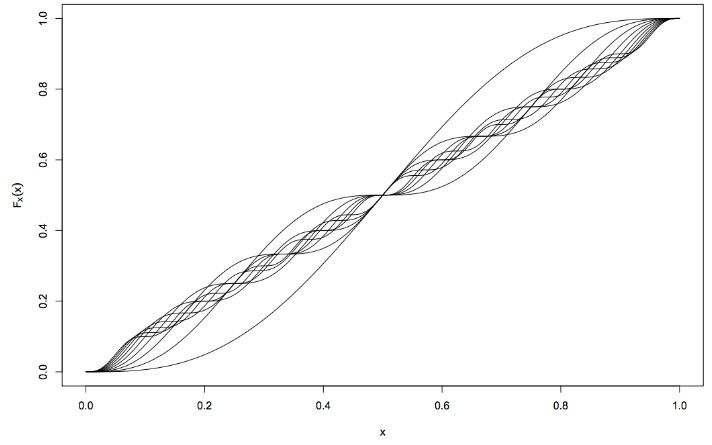
\includegraphics[width=4.5in]{conv.jpg}
\end{figure}~\spc{3}

\intermediatesubproblem{[MA] Show that $\lim_{n \rightarrow \infty} f_{X_n}$ does not exist. This is a counterexample to the conjecture that CDF convergence implies PDF convergence for finite continuous distributions with a limiting continuous distribution. Hint: it is just a calculus exercise.}\spc{2}

\end{enumerate}

\problem{These exercises will give you practice with the continuous mapping theorem (CMT) and Slutsky's theorems.}


\begin{enumerate}

\easysubproblem{State the CMT.}\spc{1}

\easysubproblem{State Slutsky's theorem A.}\spc{1}

\easysubproblem{State Slutsky's theorem B.}\spc{1}

\easysubproblem{If $X_n \convd X$ and $\lim_{n \rightarrow \infty} a_n = a$, prove $a_n X_n \convd aX$.}\spc{4}


\easysubproblem{Write the rv $S^2_n$ as a function of $\Xoneton$.}\spc{4}


\easysubproblem{Prove $S^2_n \convp \sigsq$.}\spc{10}


\easysubproblem{Prove $S_n \convp \sigma$.}\spc{1}

\easysubproblem{Prove $\sqrt{n}(\Xbar_n - \mu) / S \convd \stdnormnot$.}\spc{10}

\end{enumerate}



\problem{These exercises will introduce the Multinomial distribution. }


\begin{enumerate}


\inthenotessubproblem{If $\X \sim \multinomial{n}{\p}$ where $\dime{\X} = k$, what is the parameter space for both $n$ and $\p$?}\spc{2}

\inthenotessubproblem{If $\X \sim \multinomial{n}{\p}$ where $\dime{\X} = k$, what is $\support{\X}$?}\spc{2}

\easysubproblem{If $\X \sim \multinomial{n}{\p}$ where $\dime{\X} = k$, what is $\dime{\p}$?}\spc{-0.5}

\inthenotessubproblem{If $\X \sim \multinomial{n}{\p}$ where $\dime{\X} = 2$, express $p_2$ as a function of $p_1$.}\spc{0}

\inthenotessubproblem{If $\X \sim \multinomial{n}{\p}$ where $\dime{\X} = 2$, prove that $X_2 \sim \binomial{n}{p_2}$.}\spc{10}

\easysubproblem{If $\X \sim \multinomial{n}{\p}$ and $n = 1$ and $\dime{\X} = 7$ as a column vector, give an example value of $\x$, a realization of the r.v. $\X$. Use the notation $\bracks{\ldots}\top$ to write it as a row vector transposed.}\spc{0.5}


\easysubproblem{If $\X \sim \multinomial{n}{\p}$ and $n= 10$ and $\dime{\X} = 7$ as a column vector, give an example value of $\x$, a realization of the r.v. $\X$. Use the notation $\bracks{\ldots}\top$ to write it as a row vector transposed.}\spc{0.5}


\intermediatesubproblem{Is a binomial rv a multinomial rv? Yes or no and explain. This is subtle.}\spc{1}

%\intermediatesubproblem{If $\X \sim \multinomial{n}{\p}$ and $n= 10$ and $\p = \bracks{0.2, 0.8}^\top$, find $\muvec := \expe{\X}$.}\spc{2}


\intermediatesubproblem{If $\X \sim \multinomial{n}{\p}$ where $\dime{\X} = k$, prove that the sum over the JMF is 1. To do this, use the \href{https://en.wikipedia.org/wiki/Multinomial_theorem}{multinomial theorem}.}\spc{4}

\hardsubproblem{[MA] Let $\X_1, \X_2 \iid \multinomial{n}{\p}$ with $\dime{\X_1} = \dime{\X_2} = k$. Find the JMF of $\T_2 = \X_1 + \X_2$ from the definition of convolution. This looks harder than it is! First, use the definition of convolution and factor out the terms that are not a function of $x_1, \ldots, x_K$. Finally, use Theorem 1 in this paper: \href{https://www.researchgate.net/publication/290448343_A_combinatorial_contribution_to_the_multinomial_Chu-Vandermonde_convolution}{[click here]} for the summation.}\spc{11}

\intermediatesubproblem{Explain in English why the following should be true. Remember how the sampling from the bag works.

\beqn
\binom{n}{x_1, x_2, \ldots, x_K} = \binom{n}{x_1} \binom{n - x_1}{x_2} \binom{n - (x_1 + x_2)}{x_3} \cdot \ldots \cdot \binom{n - (x_1 + x_2 + \ldots x_{K-1})}{x_K}
\eeqn}\spc{2}

\easysubproblem{Consider the following bag of 4 green, 3 red, 2 blue and 1 yellow marbles:


\begin{figure}[htp]
\centering

\includegraphics[width=1.4in]{marbles.jpg}
\end{figure}
\FloatBarrier


Draw one marble with replacement 37 times. What is the probability of getting 10 red, 17 green, 6 blue and 4 yellow? Compute explicitly to the nearest two significant digits.}\spc{4}

\extracreditsubproblem{[MA] If $\X \sim \multinomial{n}{\p}$, find the JMF of any subset of $X_1, \ldots, X_k$. Is it technically multinomial? This is not much harder than the previous problem if formulated carefully.}\spc{8}


\easysubproblem{Consider the following rv for the remaining exercises in this problem:\\ $\X \sim \multinomial{17}{\bracks{0.1~0.2~0.3~0.4}^\top}$. What is $\dime{\X}$?}\spc{0}


\intermediatesubproblem{Find $\var{\X}$.}\spc{4}

\intermediatesubproblem{If $x_1 = 1$, what is the JDF of the remaining rv's?}\spc{4.5}

\intermediatesubproblem{If $x_1 = 1$ and $x_2 = 6$, what is the JDF of the remaining rv's?}\spc{4.5}


\easysubproblem{If $x_1 = 1$, $x_2 = 6$ and $x_3 = 3$, how is the remaining rv distributed?}\spc{3}

\end{enumerate}


\end{document}




%\easysubproblem{Prove $\expe{a\X + \c} = a\muvec + \c$ where the following are constants: $a \in \reals, \c \in \reals^K$.}\spc{2}
%
%\easysubproblem{Prove $\var{\c^\top \X} = \c^\top \Sigma \c$ where $\c \in \reals^K$, a constant and $\Sigma := \var{\X}$, the variance-covariance matrix of the vector r.v. $\X$. This is marked easy since it's in the notes.}\spc{8}

%\easysubproblem{Why is $\c^\top \Sigma \c$ called a \qu{quadratic form?} Read about it on wikipedia.}\spc{2}













%\easysubproblem{Prove the PMF of $X \sim \poisson{\lambda}$ using the limit as $n \rightarrow \infty$ and let $p = \overn{\lambda}$.}\spc{9}
%
%
%\hardsubproblem{Let $X_1 \sim \poisson{\lambda_1}$ independent of $X_2 \sim \poisson{\lambda_2}$. Find the PMF of the sum of $T = X_1 + X_2$ using a convolution.}\spc{12}

%\hardsubproblem{Let $X \sim \poisson{\lambda}$ independent of $Y \sim \poisson{\lambda}$. Find an expression for $\prob{X > Y}$ \emph{as best as you are able to answer}. Part of this exercise is identifying where you cannot go any further.}\spc{9}


%\problem{We will get some practice with the simple transformation $Y = g(X) = -X$ for discrete r.v.'s.}
%
%
%\begin{enumerate}
%
%\easysubproblem{If $X \sim \bernoulli{p}$, find the PMF of $Y = -X$. Make sure the PMF is valid $\forall y \in \reals$.}\spc{1}
%
%\easysubproblem{If $X \sim \negbin{r}{p}$, find the PMF of $Y = -X$. Make sure the PMF is valid $\forall y \in \reals$.}\spc{1}
%
%\intermediatesubproblem{If $\X \sim \multinomial{n}{\p}$, find the JMF of $\Y = -\X$. Make sure the JMF is valid $\forall \y \in \reals^K$.}\spc{1}
%
%\end{enumerate}
%
%\problem{We will now practice the conditional-on-total distributions.}
%
%\begin{enumerate}
%
%\hardsubproblem{Let $X_1, X_2 \iid \geometric{p}$ and $T = X_1 + X_2$. Find the PMF of $X_1~|~T = t$ and notate it using a brand name random variance e.g. binomial, poisson, etc. The answer may surprise you. Conditional probability is very weird!}\spc{7}
%
%
%\intermediatesubproblem{[MA] Let $X_1, X_2 \iid \binomial{n}{p}$ and $T = X_1 + X_2$. Show that $X_1~|~T = t$ is hypergeometric. You can find information about this r.v. online. Note we did not / will not study the hypergeometric further and it will not be covered on any exams.}\spc{7}
%\end{enumerate}
%
%\problem{We will now go over the Skellam distribution. In class we derived the PMF of $D = X_1 - X_2$ where $X_1, X_2 \iid \poisson{\lambda}$. This was first published in 1937. This was a special case of general Skellam distribution which is defined below:
%
%\beqn
%D \sim \text{Skellam}(\lambda_1, \lambda_2) := e^{-(\lambda_1 + \lambda_2)} \tothepow{\frac{\lambda_1}{\lambda_2}}{d/2} I_{|d|}(2 \sqrt{\lambda_1\lambda_2})
%\eeqn
%
%\noindent where $I_x(a)$ denotes the \href{https://en.wikipedia.org/wiki/Bessel_function\#Modified_Bessel_functions}{modified Bessel function of the first kind} defined as:
%
%\beqn
%I_{\alpha}(\lambda) := \sum_{x = 0}^\infty \frac{\tothepow{\overtwo{\lambda}}{2x + \alpha}}{x! (x + \alpha)!}
%\eeqn
%
%\noindent when $\alpha \in \naturals_0$.
%}\vspace{0.5cm}
%
%\begin{enumerate}
%
%\easysubproblem{Show that for $\lambda_1 = \lambda_2$, we get the formula derived in class i.e. the special case of the Skellam derived in 1937.}\spc{1}
%
%
%\intermediatesubproblem{[MA] If $D = X_1 - X_2$ where $X_1 \sim \poisson{\lambda_1}$ and $X_2 \sim \poisson{\lambda_2}$ where $X_1$ and $X_2$ are independent, show that $D \sim \text{Skellam}(\lambda_1, \lambda_2)$. You will be essentially redoing the proof published by John Gordon Skellam in 1946.}\spc{10}
%
%
%\easysubproblem{The Yankees play the Mets. Assume the number of runs scored is Poisson with rate parameter $\lambda_Y = 7$ for the Yankees and rate parameter $\lambda_M = 5$ for the Mets. Assume the number of runs scored by the Yankees is independent of the number of runs scored by the Mets. What score difference is expected in this baseball game?}\spc{2}
%
%\easysubproblem{Find the probability the Mets beat the Yankees by 3. Leave in notation. Do not compute an actual number.}\spc{2}
%
%%\easysubproblem{[MA] Figure out a way to compute the probability in the previous question to two significant figures.}\spc{1}
%
%
%\easysubproblem{Write an expression to compute the probability the Mets beat the Yankees. Leave in notation. Do not compute an actual number.}\spc{1}
%
%\end{enumerate}



%\problem{We will now practice the conditional-on-total distributions.}
%
%\begin{enumerate}
%
%\hardsubproblem{Let $X_1, X_2 \iid \geometric{p}$ and $T = X_1 + X_2$. Find the PMF of $X_1~|~T = t$ and notate it using a brand name random variance e.g. binomial, poisson, etc. The answer may surprise you. Conditional probability is very weird!}\spc{7}
%
%
%\intermediatesubproblem{[MA] Let $X_1, X_2 \iid \binomial{n}{p}$ and $T = X_1 + X_2$. Show that $X_1~|~T = t$ is hypergeometric. You can find information about this r.v. online. Note we did not / will not study the hypergeometric further and it will not be covered on any exams.}\spc{7}
%\end{enumerate}


%\problem{Introducing the king: the normal distribution $\mathcal{N}$ and his princes/sses: the lognormal distribution Log$\mathcal{N}$, chi-squared distribution $\chi^2_k$, Student's T distribution $T_k$ and Fisher-Snecodor's distribution $F_{k_1,k_2}$.}
%
%\begin{enumerate}
%
%\easysubproblem{Let $X_1 \sim \normnot{\mu_1}{\sigsq_1}$ independent of $X_2 \sim \normnot{\mu_2}{\sigsq_2}$. Prove $X_1 + X_2 \sim  \normnot{\mu_1 + \mu_2}{\sigsq_1 + \sigsq_2}$ using ch.f.'s.}\spc{5}
%
%\extracreditsubproblem{Let $X_1 \sim \normnot{\mu_1}{\sigsq_1}$ independent of $X_2 \sim \normnot{\mu_2}{\sigsq_2}$. Prove $X_1 + X_2 \sim  \normnot{\mu_1 + \mu_2}{\sigsq_1 + \sigsq_2}$ using the definition of convolution on a separate page. This is a lot of boring algebra but it will hone your skills. You can find it in the book or on the Internet (but try not to look at the answer).}\spc{-0.5}
%
%%\intermediatesubproblem{Let $X \sim \normnot{\mu}{\sigsq}$ and $Y=X ~|~X \geq a$. Find $f_Y(y)$.}\spc{6}
%
%%\easysubproblem{Let $X \sim \lognormnot{\mu}{\sigsq}$ and $Y=\natlog{X}$. How is $Y$ distributed? Use a heuristic argument. No need to actually change variables.}\spc{1}
%
%
%%\intermediatesubproblem{Let $X_1 \sim \lognormnot{\mu_1}{\sigsq_1}$, $X_2 \sim \lognormnot{\mu_2}{\sigsq_2}, \ldots, X_n \sim \lognormnot{\mu_n}{\sigsq_n}$ all independent of each other and $Y=\prod_{i=1}^n X_i$. How is $Y$ distributed? Use a heuristic argument. No need to actually change variables.}\spc{1}
%
%%\intermediatesubproblem{The average return of the S\&P 500 stock index since 1928 is 11.4\% and the standard deviation is 19.7\%. Assume for the purposes of this problem that percentage returns is normally distributed (even though it is not true in practice). If you put \$1,000 into the stock market, what is the probability you have \$5,000 after 10 years? The \texttt{R} function you need is \texttt{plnorm}.}\spc{6}
%
%
%%\easysubproblem{Using $Z_1,  Z_2, \ldots \iid \stdnormnot$, find a function $g$ s.t. $g(Z_1,  Z_2, \ldots, k_1, \ldots) \sim \chisq{k}$ where $k_1, \ldots$ represents constants.}\spc{3}
%
%\easysubproblem{Let $X \sim \chisq{k}$, find $\expe{X}$ using the fact that $X = Z_1^2 + Z_2^2 + \ldots + Z_k^2$ where $Z_1,  Z_2, \ldots, Z_k \iid \stdnormnot$.}\spc{3}
%
%\easysubproblem{Let $X \sim \chisq{k} = \gammanot{\overtwo{k}}{\half}$. Find the PDF of $X$ by making the correct substitutions in the gamma PDF and simplifying.}\spc{3}
%
%
%\easysubproblem{Using $Z_1,  Z_2, \ldots \iid \stdnormnot$, the function $g$ s.t. $g(Z_1,  Z_2, \ldots)  \sim \chisq{k}$ where $k \in \naturals$ is a constant is given below:
%
%\ingreen{
%\beqn
%g(Z_1,  Z_2, \ldots) = Z_1^2 + Z_2^2 + \ldots + Z_k^2 \sim \chisq{k}
%\eeqn}
%
%Following this example, find a function $g$ s.t. $g(Z_1,  Z_2, \ldots) \sim F_{k_1,k_2}$ where $k_1, k_2 \in \naturals$ are constants.}\spc{3}
%
%\easysubproblem{Let $X \sim F_{k_1,k_2}$, find the kernel of $f_X(x)$.}\spc{3}
%
%\easysubproblem{Using $Z_1,  Z_2, \ldots \iid \stdnormnot$, find a function $g$ s.t. $g(Z_1,  Z_2, \ldots)  \sim T_{k}$ where $k \in \naturals$ is a constant.}\spc{3}
%
%
%\easysubproblem{Let $X \sim T_k$, find the kernel of $f_X(x)$.}\spc{3}
%
%\extracreditsubproblem{Derive the PDF of the $T_k$ distribution using the ratio formula where you first find the distribution of the denominator explicitly. Do on a separate piece of paper.}\spc{0}
%
%
%\extracreditsubproblem{Show that the PDF of $X \sim T_k$, converges to the PDF of $Z \sim \stdnormnot$ when $k \rightarrow \infty$. Hint: use Stirling's approximation. Do on a separate piece of paper.}\spc{0}
%
%
%\easysubproblem{Let $X \sim \cauchynot{0}{1}$, find the kernel of $f_X(x)$.}\spc{3}
%
%\easysubproblem{Using $Z_1,  Z_2, \ldots \iid \stdnormnot$, find a function $g$ s.t. $g(Z_1,  Z_2, \ldots) \sim \cauchynot{0}{1}$.}\spc{1}
%
%\easysubproblem{Let $X \sim \cauchynot{0}{1}$, prove that $\expe{X}$ does not exist without using its ch.f.}\spc{7}
%
%
%\end{enumerate}